% swarm-cavity: results to 2026-11-26. Exploratory; not a paper.
% Build from this directory with: latexmk -pdf -halt-on-error slides.tex
% Figures: figures/*.pdf, drawn at their printed size by make_figures.py from the frozen analyses' summaries
% (sources named there). Each frame's comment names the write-up its numbers come from.
\documentclass[aspectratio=169,12pt]{beamer}
\usepackage[T1]{fontenc}
\usepackage{lmodern,tgpagella,tgheros}
\usepackage{amsmath,array,graphicx,tikz}
\usetikzlibrary{arrows.meta}
\usefonttheme[onlymath]{serif}
\definecolor{ink}{gray}{0.09}
\definecolor{secondary}{gray}{0.33}
\setbeamercolor{normal text}{fg=ink,bg=white}
\setbeamercolor{structure}{fg=ink}
\setbeamercolor{frametitle}{fg=ink,bg=white}
\setbeamerfont{title}{family=\rmfamily,series=\bfseries}
\setbeamerfont{frametitle}{parent=title,size=\Large}
\setbeamerfont{section title}{parent=title}
\setbeamerfont{subsection title}{parent=title}
\setbeamerfont{block title}{family=\rmfamily,series=\bfseries}
\setbeamersize{text margin left=9mm,text margin right=9mm}
\setbeamertemplate{navigation symbols}{}
\setbeamertemplate{headline}{}
\setbeamertemplate{footline}{}
\setbeamertemplate{frametitle}{%
  \vspace*{4mm}\noindent\usebeamerfont{frametitle}\insertframetitle\par}
\newcommand{\contextline}[1]{{\footnotesize\color{secondary}#1\par}}
\newcommand{\sidenote}[1]{{\footnotesize #1\par}}
\hypersetup{pdftitle={Cavity theory of LLM agent swarms: the reaction term, measured},pdfauthor={}}

\begin{document}

% Theory and protocol. Field: theory/claim1.md eq. (4). Echo: theory/quiet_regime.md eq. (K2) and the sign table of
% section 3.2. Protocol: section 3.1 (envs/kick.py).
\begin{frame}{An echo needs a reciprocated tie}
  \begin{columns}[c,onlytextwidth]
    \begin{column}{.37\linewidth}
      \centering
      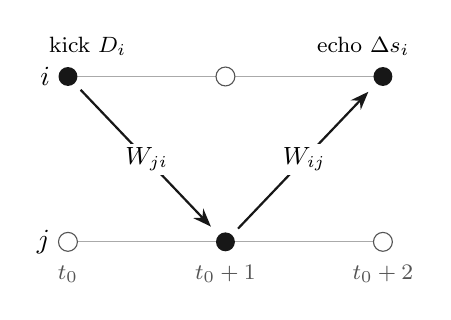
\begin{tikzpicture}[x=1cm,y=1cm,>=Stealth,
          site/.style={circle,inner sep=0pt,minimum size=2.4mm,fill=ink},
          ghost/.style={circle,inner sep=0pt,minimum size=2.4mm,draw=secondary,fill=white},
          hop/.style={->,shorten <=3pt,shorten >=4pt,draw=ink,thick}]
        \foreach \y in {0,2.1}{\draw[secondary!50,thin] (0,\y) -- (4,\y);}
        \foreach \x/\t in {0/{t_0},2/{t_0+1},4/{t_0+2}}{
          \node[below=5pt,secondary] at (\x,0) {\footnotesize$\t$};}
        \node[site] (i0) at (0,2.1) {};  \node[ghost] at (2,2.1) {};   \node[site] (i2) at (4,2.1) {};
        \node[ghost] at (0,0) {};        \node[site] (j1) at (2,0) {}; \node[ghost] at (4,0) {};
        \node[left=3pt] at (0,2.1) {$i$};
        \node[left=3pt] at (0,0) {$j$};
        \draw[hop] (i0) -- node[midway,fill=white,inner sep=1.5pt] {\small$W_{ji}$} (j1);
        \draw[hop] (j1) -- node[midway,fill=white,inner sep=1.5pt] {\small$W_{ij}$} (i2);
        \node[above=4pt] at (0.25,2.1) {\footnotesize kick $D_i$};
        \node[above=4pt] at (3.75,2.1) {\footnotesize echo $\Delta s_i$};
      \end{tikzpicture}\par
      \vspace{3mm}
      \contextline{\raggedright Twin runs: restore a finished run at round $t_0$, mirror agent $i$'s message
        as its readers $j$ see it ($p\to1-p$), and replay two rounds.}
    \end{column}
    \begin{column}{.59\linewidth}
      \small
      Cavity field on agent $i$: mean, noise, reaction.
      \[
        h_i(t)=\bar J\,m(t)+\eta_i(t)+\Gamma\sum_{t'<t}R(t,t')\,s_i(t')
      \]
      The kick enters through the reaction term alone:
      \[
        \Delta s_i(t_0+2)=d_i\!\sum_{j:\,i\rightleftarrows j}\! W_{ij}\,d_j\,W_{ji}\;D_i ,
        \qquad d=1-s^2 ,
      \]
      with $W=+a_+/K$ on an agree tie, $-a_-/K$ on a disagree tie.
      \par\vspace{2.5mm}
      \renewcommand{\arraystretch}{1.2}
      \begin{tabular}{@{}l@{\quad}l@{}}
        $\gamma=0$: no tie reciprocated & echo exactly $0$ \\
        $\gamma>0$: equal signs & $W_{ij}W_{ji}>0$ \\
        $\gamma<0$: opposite signs & $W_{ij}W_{ji}=-a_+a_-/K^2$
      \end{tabular}
    \end{column}
  \end{columns}
\end{frame}

% Kick stage 1. experiments/07_kick/RESULT.md, rule 1; results/kick1k-20261125-summary.json; figure block 1.
\begin{frame}{One prompt sentence flips the echo's sign}
  \centering
  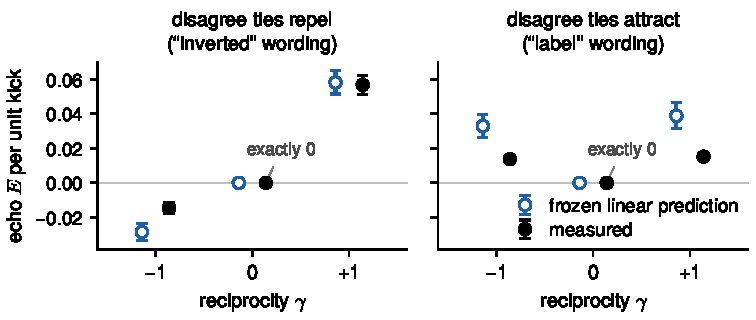
\includegraphics[width=128mm]{figures/echo_sign.pdf}\par
  \smallskip
  \contextline{Haiku 5.5, $N=64$, $K=2$, 8 graphs per cell. 7,146 kick twins at $\gamma=\pm1$; all 878 at
    $\gamma=0$ give exactly zero. The panels share graphs, evidence and kicks. Bars: 1 s.e.}
\end{frame}

% Kick stage 2. RESULT_stage2.md, rules 1, 2, 6; results/kick2-additivity.json; figure block 2.
\begin{frame}{Echoes add over ties and persist at $K=4$}
  \centering
  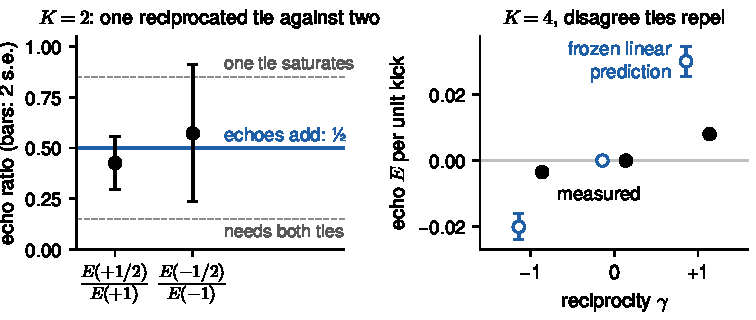
\includegraphics[width=128mm]{figures/additivity_k4.pdf}\par
  \smallskip
  \contextline{New graphs, 7,036 twins. Ratio $0.43\pm0.07$ against $\tfrac12$. The $K=4$ echoes have the
    predicted sign at 3.5 and 6.7 s.e., and are 4 to 6 times smaller than predicted.}
\end{frame}

% Magnitude. RESULT.md rule 4 and RESULT_stage2.md rule 6; predictions quiet_regime.md section 3.8; figure block 3.
\begin{frame}{Calibrated gains overstate settled agents}
  \begin{columns}[c,onlytextwidth]
    \begin{column}{80mm}
      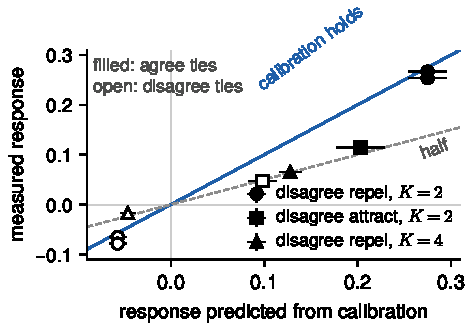
\includegraphics[width=80mm]{figures/first_order.pdf}
    \end{column}
    \begin{column}{56mm}
      \raggedright
      \sidenote{Response of a reader to one flipped message, per unit kick.}
      \medskip
      \sidenote{The calibration probed fresh agents reading a whole new inbox. A kick reaches a settled agent
        and changes one of its $K$ messages.}
      \medskip
      \sidenote{Composing the measured responses reproduces the echoes, within a factor 1.4 at $K=4$.
        The structure of the reaction term holds; its size needs gains measured on settled agents.}
    \end{column}
  \end{columns}
\end{frame}

% Asymmetry. RESULT.md (unplanned finding), RESULT_stage2.md rules 5 and 7; figure block 4.
\begin{frame}{Confirming inputs move agents less}
  \centering
  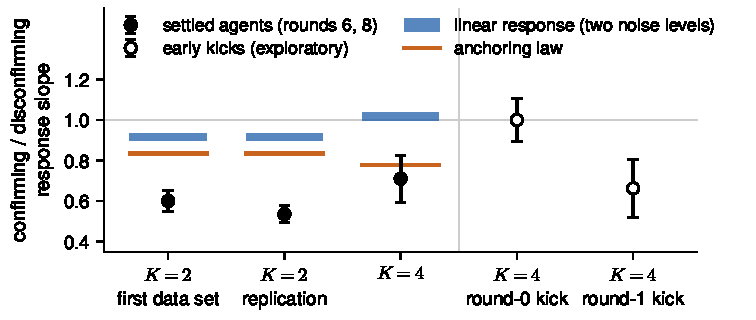
\includegraphics[width=128mm]{figures/asymmetry.pdf}\par
  \smallskip
  \contextline{Response slope to a second-step input that pushes an agent along its lean, over the slope for an
    input against it. Unplanned in the first data set; the replication was pre-registered.}
\end{frame}

% Where the swarms sit. quiet_regime.md section 2.1; 06-qwen-calibration, 08 and 08b RESULT.md; figure block 5.
\begin{frame}{Every swarm sits far from the instability}
  \centering
  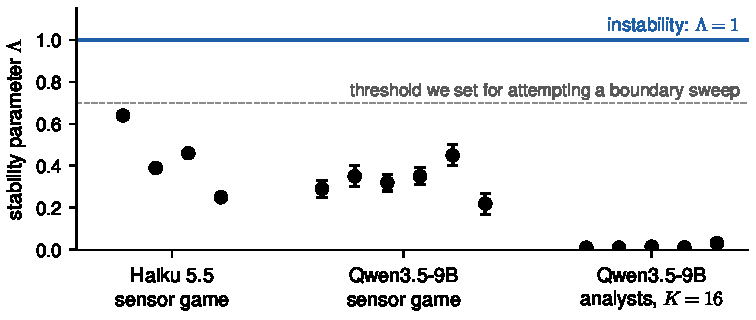
\includegraphics[width=128mm]{figures/stability.pdf}\par
  \smallskip
  \contextline{One point per wording and $K$. $\Lambda=d\,g\,(1+|\gamma_{\rm eff}|)$ from measured gains; for
    analysts, the solver's value. The transition and the zealot hysteresis remain untested.}
\end{frame}

% Analyst calibrations (no-go). experiments/08-analyst-calibration and 08b RESULT.md; figure block 6.
\begin{frame}{Distrusted colleagues still attract}
  \centering
  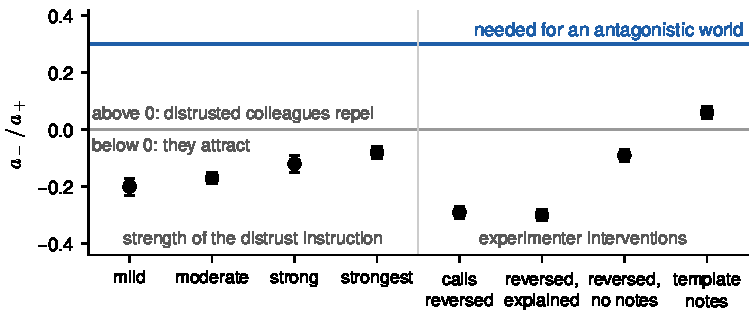
\includegraphics[width=128mm]{figures/analyst_fade.pdf}\par
  \smallskip
  \contextline{Qwen3.5-9B analysts make BUY/SELL calls and read 16 colleagues: 8 allies, 8 marked ``usually
    wrong''. $a_+$: pull toward allies. $a_-$: push away from distrusted colleagues.}
\end{frame}

% Sign-rule test. experiments/09-analyst-signrule/RESULT.md; theory/analyst_signrule.md eq. (S5); figure block 7.
\begin{frame}{On Qwen, the echo again needs reciprocity}
  \begin{columns}[c,onlytextwidth]
    \begin{column}{80mm}
      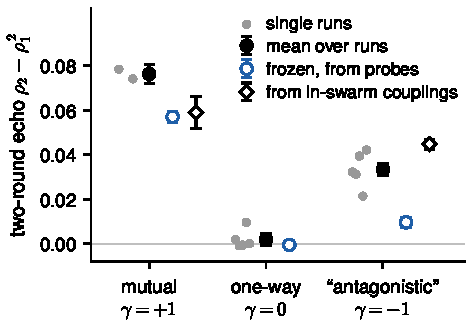
\includegraphics[width=80mm]{figures/signrule_echo.pdf}
    \end{column}
    \begin{column}{56mm}
      \raggedright
      \sidenote{Kick twins agree: $+0.069\pm0.014$, $0$, $+0.031\pm0.007$.}
      \medskip
      \sidenote{Distrusted colleagues attract, so the rule predicts a positive ``antagonistic'' echo.
        In the swarm they attract three times more than in probes, which sets its size.}
      \medskip
      \sidenote{\color{secondary}An effect blind to tie signs would give the same signs.}
    \end{column}
  \end{columns}
  \smallskip
  \contextline{$N=256$, $K=16$, 20 rounds, 12 runs. Calls are sampled by the experimenter with the SELL bias
    removed. $\rho_k$: lag-$k$ autocorrelation of an analyst's call.}
\end{frame}

% Asynchronous control. 09 RESULT.md, falsifier 7; theory/analyst_signrule.md Amendment 1; figure block 8.
\begin{frame}{Asynchrony moves the echo to lag 1}
  \begin{columns}[c,onlytextwidth]
    \begin{column}{80mm}
      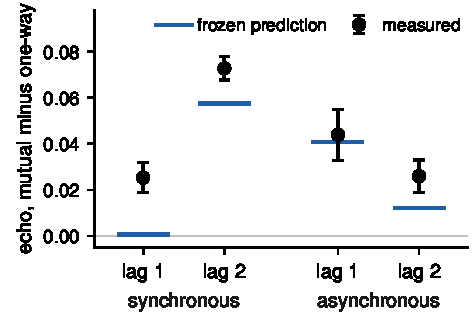
\includegraphics[width=80mm]{figures/signrule_async.pdf}
    \end{column}
    \begin{column}{56mm}
      \raggedright
      \sidenote{Each round, 16 random blocks of 16 analysts update in turn, so a reply can return within the
        round.}
      \medskip
      \sidenote{Lag 1 appears as predicted: $+0.044\pm0.011$ against $+0.041$.}
      \medskip
      \sidenote{Lag 2 fell to 0.36 of its synchronous value, against 0.21 predicted. The pre-registered test is
        unresolved at 1.4 s.e.}
    \end{column}
  \end{columns}
  \smallskip
  \contextline{Predictions frozen before any asynchronous run; 4 mutual and 4 one-way runs. Not predicted: the
    synchronous lag-1 contrast, which comes from 2 mutual runs.}
\end{frame}

% Decision frame. HANDOFF.md, "Next"; RESULT_stage2.md rule 3 (K = 2 discount) and its closing section.
\begin{frame}{What should the next measurement be?}
  \footnotesize
  \renewcommand{\arraystretch}{1.55}
  \begin{tabular}{@{}>{\raggedright\arraybackslash}p{50mm}@{\hspace{6mm}}>{\raggedright\arraybackslash}p{84mm}@{}}
    {\small\rmfamily\bfseries Does an agent discount its own returning influence?} &
      At $K=2$ a returning change moved agents 20\% less than a matched change from elsewhere
      ($-0.18\pm0.04$). One data set, not pre-registered. \\
    {\small\rmfamily\bfseries Is the asymmetry a single-agent property?} &
      Probe single agents with matched confirming and disconfirming changes, settled and fresh.
      Round-0 kicks showed none ($1.00\pm0.11$). \\
    {\small\rmfamily\bfseries Can echo sizes be predicted in advance?} &
      Measure gains on settled agents with one message flipped, per wording and $K$. \\
    {\small\rmfamily\bfseries Where is a strongly coupled swarm?} &
      The transition and hysteresis predictions need $\Lambda$ near 1. Nothing in hand reaches 0.7.
  \end{tabular}
  \par\vfill
  \contextline{Spend so far: \$146 of \$2,000. The first three are cheap on Haiku; the fourth is a search.}
  \vspace{4mm}
\end{frame}

\end{document}
